
\documentclass{beamer}
\usepackage[latin1]{inputenc}
%\usetheme{Montpellier}
%\usetheme{Boadilla}
%\usecolortheme[RGB={204,51,255}]{structure}
%\usecolortheme[named=purple]{structure}
\usecolortheme[RGB={62,128,62}]{structure}
%\definecolor{reddish}{rgb}{0.3,0.15,0.3}
%\definecolor{light}{rgb}{0.8,0.6,0.8}
%\definecolor{reddish}{rgb}{.5,0.15,0.15}
\definecolor{reddish}{rgb}{0.5,0.3,0.4}
%\definecolor{light}{rgb}{0.8,0.6,0.8}
\definecolor{reddish}{rgb}{.7,0.25,0.25}
\definecolor{greenish}{rgb}{.25,0.7,0.25}
\definecolor{blueish}{rgb}{.25,0.25,0.7}
\definecolor{purple}{rgb}{.5,0.0,0.5}
\usepackage{graphicx}
\usepackage{pstricks}

\newcommand{\btVFill}{\vskip0pt plus 1filll}

\setbeamertemplate{navigation symbols}{}

\newcommand{\crish}{\color{reddish}}
\newcommand{\cbla}{\color{black}}
\newcommand{\cred}{\color{red}}
\newcommand{\cblu}{\color{blue}}
\newcommand{\cgre}{\color{green}}

\newcommand{\sm}{\color{reddish}$}
\newcommand{\fm}{$\color{black}{}}

\newcommand{\letter}[1]{\color{blue}\texttt{#1}\color{black}}
\newcommand{\binary}[1]{\color{red}\texttt{#1}\color{black}}

\usepackage{tikz}
\usetikzlibrary{arrows,decorations.markings,positioning}
\usepackage{epstopdf}
\usetikzlibrary{fit}

\title[Information Theory task 3]{Gambling}
\author{COMSM0075 Information Processing and Brain}
\institute{\texttt{comsm0075.github.io}}
\date{October 2020}

\begin{document}

\maketitle


\begin{frame}{Gambling}
Gambling presents a set of useful `toy examples' for considering the
role of information in decision making and strategy.
\end{frame}


\begin{frame}{Gambling}
Do not gamble - you will lose all your money!
\end{frame}



\begin{frame}{A sulky race}
  \begin{center}
    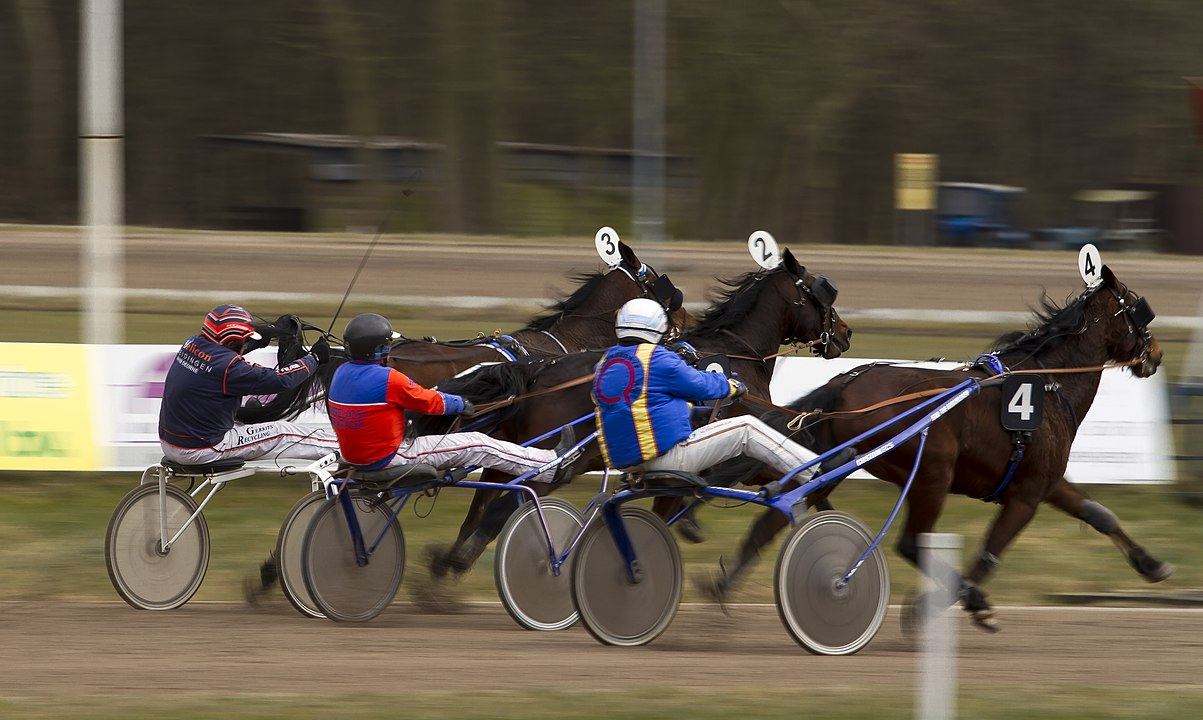
\includegraphics[width=8cm]{sulky_racing.jpg}
  \end{center}
  \vfill
  \flushright{\tiny{\cred{}Image from wikipedia\cbla{}}}
\end{frame}

\begin{frame}{A race}
\crish$n$\cbla{} outcomes corresponding to \crish$n$\cbla{} different
potential winners. Each outcome has some probably unknown probability
\crish$p_a$\cbla.
\end{frame}

\begin{frame}{Odds}
  \begin{center}
    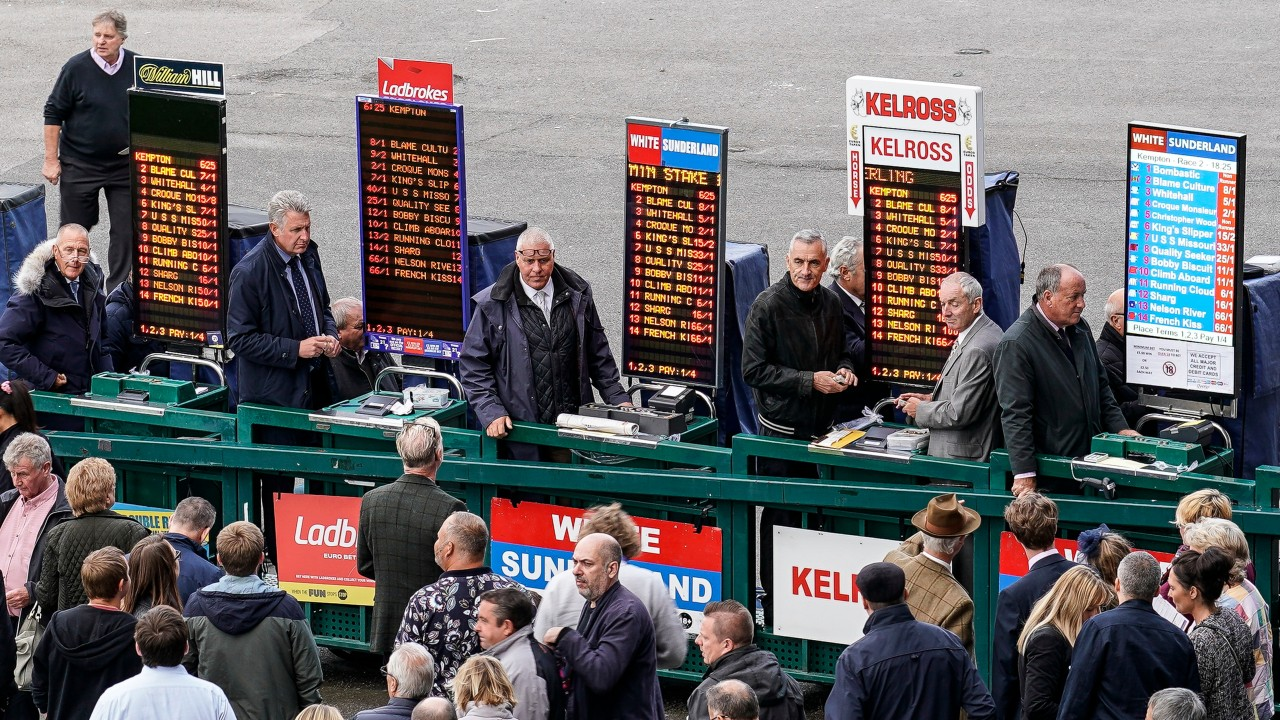
\includegraphics[width=4cm]{bookies.jpg}
  \end{center}
The bookie will offer \textbf{odds}; we will use
\crish$r_a$\cbla{} the amount paid out for each euro bet, so if you
bet \crish$A$\cbla{} on horse \crish$a$\cbla{} and it won, you would get
\crish$Ar_a$\cbla{} back.
\end{frame}

\begin{frame}{Odds}
  \begin{center}
    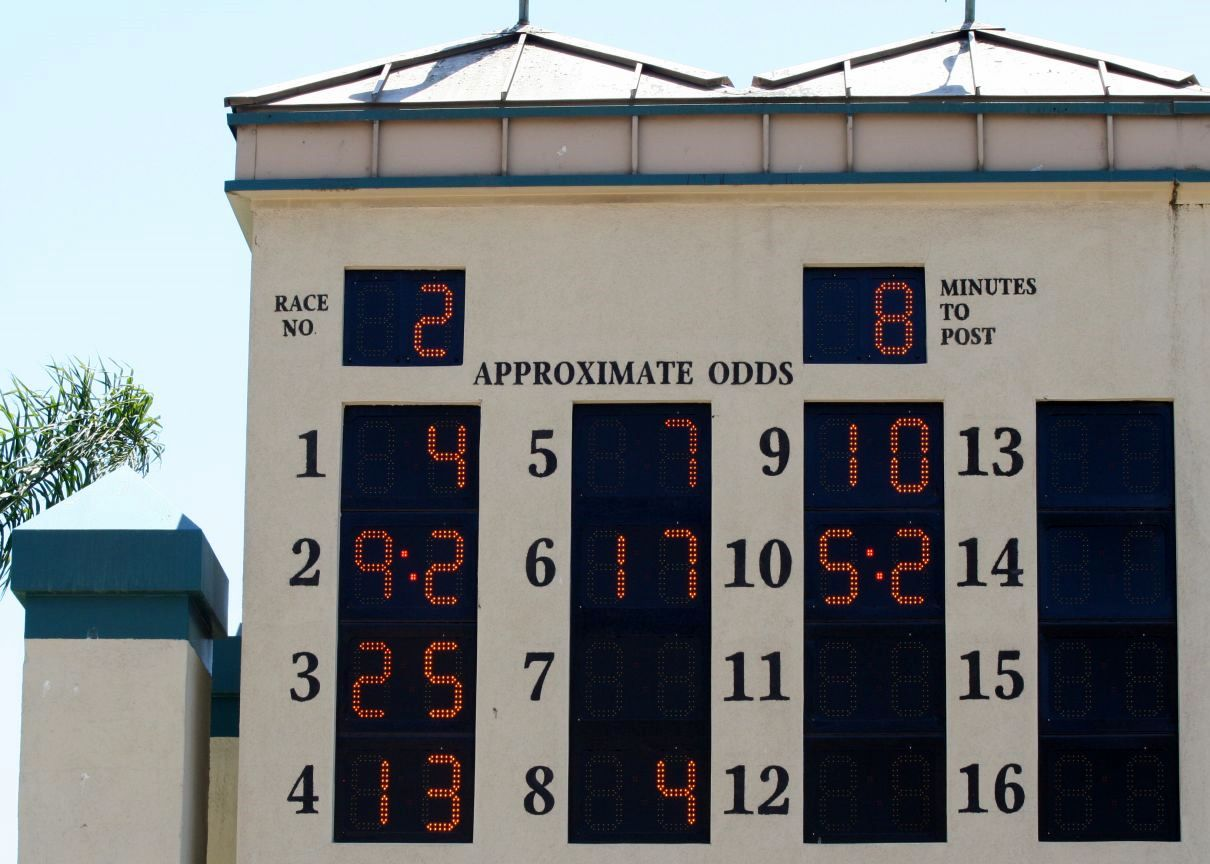
\includegraphics[width=4cm]{tote.jpg}
  \end{center}
Odds of \crish{}5/2\cbla{} means if you get bive and win you get your five back and two extra giving you seven in total, so that's equivalent to \crish$r=7/5$\cbla{}.
\end{frame}

\begin{frame}{Gambling strategy}
\begin{quote}
Should you bet everything on the horse you think mostly likely to win or should you spread your bets around.
  \end{quote}
\end{frame}

\begin{frame}{Gambling strategy}
\begin{quote}
  As a simplified problem, imagine we are intending to bet repeatedly on the same race and we are intending to go \textbf{all in} every time. 
\end{quote}
Your gambling strategy is how you spread you bets across the
horses. Let \crish$b_a$\cbla{} be the fraction of your total cash you bet
on the \crish$a$\cbla{}th horse. The vector \crish$\mathbf{b}$\cbla{}
is your \textbf{gambling strategy} with \crish$\sum_ab_a=1$\cbla{}.
\end{frame}
   

\begin{frame}{Earnings - one race}
Your total amount of cash is your \textbf{float}; in this simplied
version you always bet all your float.
\vskip 1cm
Recall \crish$b_a$\cbla{} be
the fraction of your float you bet on the \crish$a$\cbla{}th horse. If
\crish$A$\cbla{} was your float and the horse \crish$w$\cbla{} wins you will have
\crish$$S(w)A=b_wr_wA$$\cbla{} after the race.
\end{frame}


\begin{frame}{Earnings - one race}
So ratio of your float afterwards to your float before is
\crish$$S(w)=b_wr_w$$\cbla{} after the race if \crish$w$\cbla{} wins. We can think of this as a random variable \crish$S$\cbla{} which is a function of the random variable \crish$W$\cbla, the winner: \crish$S(W)$\cbla{}.
\end{frame}


\begin{frame}{Earnings - many races}
If there are \crish$N$\cbla{} races then at the end of the day you will have \crish$$
S_N=\prod_{i=1}^N S(w(i))=\prod_{i=1}^N b_{w(i)}r_{w(i)}
  $$\cbla{}where \crish$w(i)$\cbla{} is the winner of the
  \crish$i$\cbla{}th race and we are setting the initial float to one.
\end{frame}
   

\begin{frame}{The doubling rate}
  The \textbf{doubling rate} is defined as
  \crish
  $$
  R(\mathbf{p},\mathbf{b})=\langle \log_2{S(W)}\rangle= \sum_a{p_a\log_2{b_ar_a}}
  $$
  \cbla
\end{frame}

\begin{frame}{Why the `doubling rate'?}
  Assume the results \crish$\{W_1,W_2,\ldots,W_N\}$\cbla{} are independent and have the same distribution, then if we bet with strategy \crish$\mathbf{b}$\cbla{} we have
  \crish
  $$ \frac{1}{N}\log_2{S_N}=\frac{1}{N}\sum_i \log_2{b_{w(i)}r_{w(i)}}\rightarrow \langle \log_2{b_{w(i)}r_{w(i)}}\rangle_W= R(\mathbf{p},\mathbf{b})$$
  \cbla
  so\cblu
  $$
  S_N\approx 2^{NR(\mathbf{p},\mathbf{b})}
  $$\cbla
\end{frame}

\begin{frame}{Best strategy}
  We want to maximize \crish$R(\mathbf{p},\mathbf{b})$\cbla{} over all choices of \crish$\mathbf{b_i}$\cbla{} subject to the constraint that \crish$b_a\ge0$\cbla{} and \crish$\sum_ab_a=1$\cbla{}. For a constrained optimization we use a Lagrange multiplier:
  \crish $$
  J=\sum \sum_a{p_a\log_2{b_ar_a}} +\lambda \sum_ab_a
  $$\cbla
  Now
  \crish $$
  \frac{dJ}{db_a}=\frac{p_a}{b_a}+\lambda
  $$\cbla
  and, for a stationary point \crish$dJ/db=0$\cbla{} so
    \crish $$
  p_a=-\lambda b_a
  $$\cbla
  Finally sum over \crish$a$\cbla{}:
    \crish $$
  \sum_a p_a = -\lambda \sum_a b_a
  $$\cbla
  giving \crish $\lambda=-1\cbla{}$\cbla{} and
  \crish $$
  b_a=p_a
  $$\cbla
\end{frame}

\begin{frame}{Proportional betting is best}
  \crish $$
  b_a=p_a
  $$\cbla
\end{frame}

\begin{frame}{In fact}
  \crish
  $$
  R(\mathbf{p},\mathbf{b})= \sum_a{p_a\log_2{b_ar_a}}=\sum_a{p_a\log_2{\frac{b_a}{p_a}p_ar_a}}
  $$
  \cbla  
  then splitting the log
  \crish
  $$
  R(\mathbf{p},\mathbf{b})=\sum_ap_a\log_2{\frac{b_a}{p_a}}+\sum_ap_a\log_2{p_ar_a}
  $$
    \cbla
    and splitting the second term again this give
    \crish
    $$
      R(\mathbf{p},\mathbf{b})=\sum_ap_a\log_2{r_a}-H(\mathbf{p})-D(\textbf{p}\|\textbf{b})
      $$\cbla
and since the first two terms don't depend on \crish$r_a$\cbla{} this shows that proportional betting is the best strategy. 
\end{frame}


\begin{frame}{The cost of ignorance}
\crish
  $$
      R(\mathbf{p},\mathbf{b})=\sum_ap_a\log_2{r_a}-H(p)-\cblu{}D(\textbf{p}\|\textbf{b})
      $$
\cbla
\end{frame}

\begin{frame}{If the odds are fair}
  Say
  \crish
  $$
  \sum_a\frac{1}{r_a}=1
  $$
  \cbla{}
  then
\crish
  $$
      R(\mathbf{p},\mathbf{b})=\cgre{}D(\textbf{p}\|\textbf{r})\crish{}-\cblu{}D(\textbf{p}\|\textbf{b})
      $$
      \cbla
and betting is a competition of knowledge between you and the bookie.      
\end{frame}

\begin{frame}{The Kelly criterion - a question}
 The \textbf{Kelly criterion} is an investment strategy which can be
 derived in its simplest form using the methods we have discussed. In
 a simple example you have the opportunity to bet on event, that two
 dice roll a seven for example. If your bet is a success you get
 \crish$r$\cbla{} times your stake, if it fails you get nothing. The
 probability of success is \crish$p$\cbla. What fraction of your float
 should you bet each time?
\end{frame}


\end{document}

